% !TEX root = ../thesis-main.tex

\chapter{Introduction}
\label{chapter:introduction}

% aided by this chatGPT conversation: https://chat.openai.com/share/2cbbe97e-207c-4cfb-8558-c576a155814a
% and this BING chat conversation: https://sl.bing.net/M0SlEtfmSG, https://sl.bing.net/f7cUBW51tam

Video streaming platforms have changed the way people consume and interact with digital media~\cite{NetflixReco}. 
One of the key innovations of video streaming platforms with regards to traditional television, is \emph{personalization}, that is, the ability to tailor the experience to each single user and their interests, given their past behavior on the platform~\cite{oldPersonalizationBehavior, oldPersonalizationSearch}. 

\begin{figure}[t]
  \captionsetup{singlelinecheck=off}
  \centering
  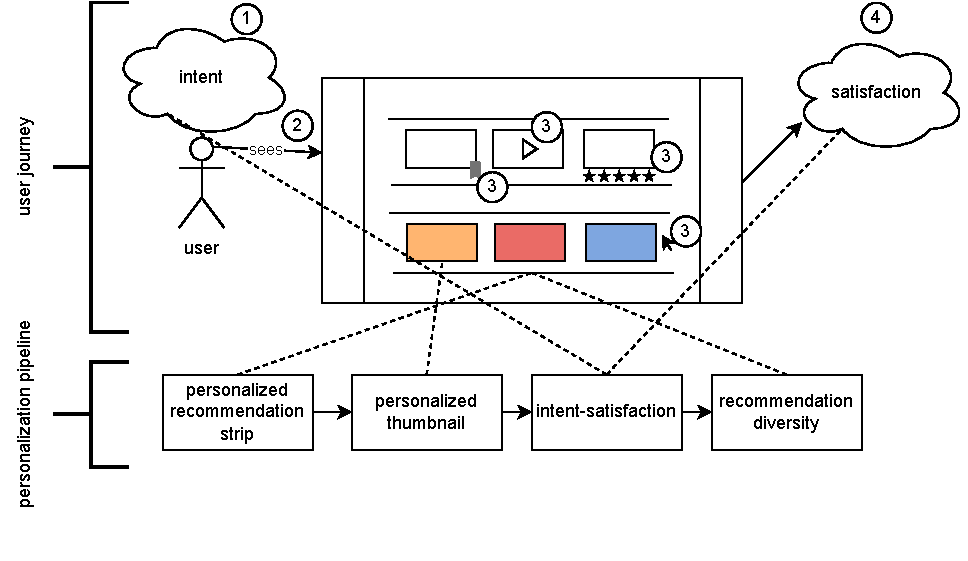
\includegraphics[width=\textwidth]{images/personalization_pipeline.pdf}
  \caption[a]{Our \emph{user journey} and \emph{recommendation pipeline} paradigm.
    Along the \emph{user journey}, a user 
    \begin{enumerate*}[label={(\arabic*)}]
    \item has an intent (e.g., series catch up)
    \item sees the home page with video thumbnails inside recommendation strips
    \item interacts with the platform (clicks, scrolls, bookmarks, video plays, ratings, etc.)
    \item feels a certain level of (dis)satisfaction with the platform over time.
    \end{enumerate*}
    With the \emph{recommendation pipeline}, the platform
    \begin{enumerate*}[label={(\roman*)}]
    \item generates personalized strips
    \item selects personalized thumbnails (stills from a video)
    \item measures the relationship between intent, interactions and satisfaction
    \item measures the appropriate level of content diversity.
    \end{enumerate*}}
  \label{fig:journey}
\end{figure}

When designing and examining methods for personalization, the concept of \emph{user journey} is helpful. 
We propose this term in the context of this thesis to describe the user's interactions with a video streaming platform from login to logout.
In the setting of video streaming, the user journey consists of several steps (see Figure~\ref{fig:journey}).
First, users come to the platform with some \emph{intents} (e.g., binge-watching a series, finding a family-friendly movie, discovering new genres)~\cite{intent}. 
Then, they see a customized home page with various horizontal \emph{recommendation} strips.
In Figure~\ref{fig:VLStrip} we show how this step in the user journey is realized with the landing page of Videoland, a Dutch video-on-demand service. 
Each strip contains videos with (sometimes personalized) \emph{thumbnails} (the clickable image that represents the video content). 
Over time, users interact with the platform and leave \emph{behavioral} signals (e.g., clicks, watch time, bookmarks, ratings, etc.). 
From the platform's perspective, deciphering how these behavioral signals, prompted by user intents, translate into overall \emph{satisfaction} remains a complex challenge~\cite{spotifyIntent}.

Behavioral signals generated during the user journey have long been drawn on to target users individually. 
The term \emph{personalization} is commonly used to describe this strategy. 
Historically, personalization has been used as an umbrella term for approaches more akin to targeting user segments/groups than actually serving each single user differently (as the term personalization seems to hint at). 
Initially, in the domain of e-commerce in the late 1990s, personalization was restricted to email newsletters and aimed at user groups~\cite{oldReco}. 
Personalization appeared on early video streaming platforms like Netflix in the form of one-dimensional lists, i.e.,  the recommendation strip mentioned above~\cite{oldReco}. 
Today, the user journey on video platforms is steered by the platform's algorithms: personalization is used in the ordering of the strip (i.e., multiple one-dimensional lists, in the choice of the thumbnail, in the font title of the thumbnail, in search (a review of these strategies can be found in~\cite{NetflixReco}).

\begin{figure}[t]
  \centering
  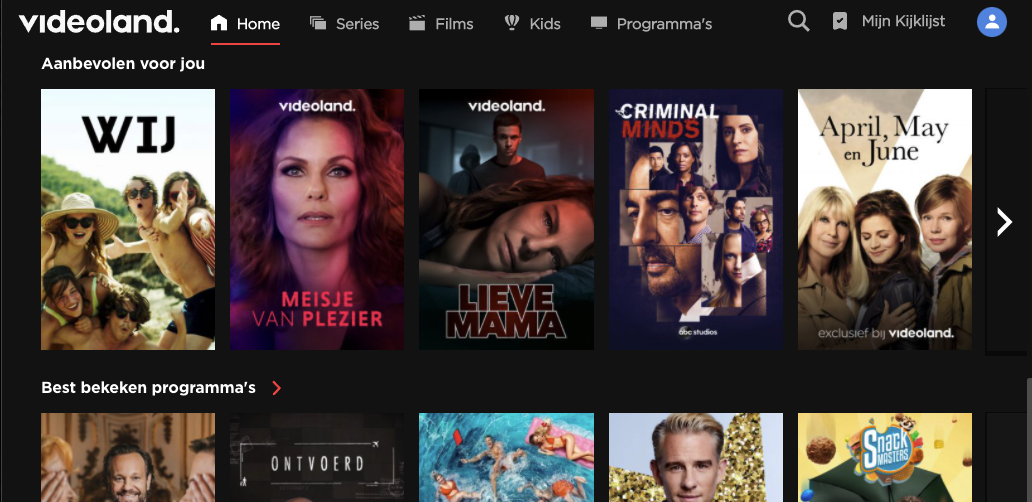
\includegraphics[width=\textwidth]{images/VLHome_cropped.png}
  \caption{Videoland's recommendation strips}
  \label{fig:VLStrip}
\end{figure}

In this thesis, the term \emph{personalization pipeline} is used to denote the accumulation of a video platform's algorithms for a tailored user journey (see Figure~\ref{fig:journey}). 
One part of the pipeline retrieves data that feeds all other algorithms: collecting user data and analyzing user behavior~\cite{behaviorals}.
% These signals, also called user feedback are often provided by an external analytics business and the signal granularity is limited by the amount of data and how much a streaming platform is willing to pay \tocite{}.
The data granularity can range from the number of items watched (just one data point per user session), all the way to recordings of all mouse movements (thousands of data points per session). With that session-level data, streaming platforms attempt to predict what the user will do and adapt the user journey to the user: the next movie to watch, the subsequent logins, the midterm satisfaction (typically, the amount of time spent on the platform per month), all the way to churn rate (subscription cancellation rate)~\cite{longTerm}; from short to long term forecast. These predictive models are tested first on a simulated platform with simulated users ``offline.'' 
Models are then evaluated on the platform exposed to users ``online'' over several iterations and over time. In the evaluation phase, preferences, and interaction patterns are captured again as a feedback loop~\cite{offlineOnlineSurvey, NetflixReco}. 

Aside from the measurable user feedback signals (such as clicks, watch time, time on the platform, etc.), a platform can also take hidden signals into consideration. In this thesis, we give some attention to user intent (``I want to watch the next episode of my favorite show,'' ``I am looking for new content,'' ``I want to bookmarking items for later viewing,'' etc.). 

Besides satisfying the users, the platform also bears another responsibility, because it is able to steer the user towards certain consumption behaviors. For example, the platform has to ensure that the content it offers is \emph{diverse} and promotes representative voices (e.g., promoting screenwriters of different genres, movies in different languages, a variety of movie genres). %These concerns are revisited below via our own personalization pipeline.

For the purpose of this thesis, we will call the combination of algorithms listed above the \emph{personalization pipeline}. 
This pipeline is often geared towards optimizing relatively simple metrics like the number of minutes seen~\cite{spotifyIntent} and the churn rate~\cite{oldChurn}, but it is also directly linked to a responsibility to balancing multiple, sometimes competing targets, such as long-term user satisfaction~\cite{longTerm}, content diversity, and  ethical considerations~\cite{helberger}.

%regarding satisfaction and diversity are related to the platform's perspective.
%building predictive models, testing different strategies, and evaluating the outcomes. These steps help to capture user intent, preferences, and interaction patterns; the input for personalization tools. This thesis presents some novel methods and tools for improving the pipeline along this user journey. 

In this thesis, we propose individual tools that use the logged interactions from the user journey above, for the steps of \emph{recommendations}, \emph{thumbnail} selection, \emph{intent-satisfaction} linking, and \emph{diversity} measurement. 
Together, these tools form our proposed personalization pipeline. In the thesis we seek to make novel contributions to each of the steps in the personalization pipeline as depicted in Figure~\ref{fig:journey}.
By adapting diffusion models~\cite{jascha} from the image domain (continuous-2D-structured-data) to recommendation (binary-1D-unstructured-data), we open the door to the use of priors in recommendation (preferred movie genres, past behavior or incomplete viewing history, etc.), like is seen in diffusion for images (an image description, a previous reference image, a masked image, etc.) \todo{REF}. Diffusion models are physics inspired neural models, that include a forward (perturbation) and backward (learning) process on each example~\cite{jascha}. \mdr{Why do we need this particular detail about diffusion at this stage?} As for personalized \emph{thumbnails}, existing research in multilabel image classification is highly reliant on variations of the binary cross-entropy loss~\cite{fisher}, but we think that the multilabel setting (as opposed to the binary or multiclass setting) requires its own solution. For the next step, we identified a lack of a systematic approach for \emph{intent-satisfaction} studies, that would provide survey design, code and modern bayesian approaches to the problem. 
Finally, we argue for the importance of a \emph{diversity} metric for news / movies recommendations that is distribution agnostic -- to adapt to any distributions of discrete normative standpoints -- and rank-aware -- to accommodate for the propensity of a user to scroll up to an item on a ranked list. 
As such a metric is missing from the literature, we propose a rank-aware adaptation of the Jensen-Shannon Divergence.

%We identify a knowledge gap in the literature 
%\paragraph{knowledge gap...} list for each paper.
%The tools we propose here are: a generative model for creating diverse and relevant recommendation strips for the home page; a multilabel classifier for selecting optimal thumbnails for each video; a survey-based method for predicting user satisfaction from intent and behavior; and a set of metrics for measuring content diversity and avoiding unwanted biases.

In short, in this thesis, I focus on the video streaming platform ecosystem, explore the challenges and opportunities of personalization, recommendation, and user behavior analysis. 
By combining survey methods, modeling, adaptive testing, and behavioral analysis, this study aims to contribute to the development of video streaming platforms that can provide user satisfaction in a responsible way.

%% The research questions and sub questions
% !TEX root = ../thesis-main.tex

\acrodef{rq:recfusion}[\ref{rq:recfusion}]{Can we use diffusion to do recommendation in the classical user-item matrix setting?}

\acrodef{rq:sigmoidf1}[\ref{rq:sigmoidf1}]{Is there a way we can generate personalized thumbnails for each item on a streaming platform?}

\acrodef{rq:intent}[\ref{rq:intent}]{Are users' intents together with their behavioral data useful signals to predict or explain satisfaction on a video streaming platform?}

\acrodef{rq:radio}[\ref{rq:radio}]{Can we formulate a divergence metric that measures the normative diversity of recommendations?}

\section{Research Outline and Questions}
\label{section:introduction:rqs}


We scope the thesis around four research questions, each corresponding to a chapter in the thesis.

% https://sl.bing.net/c5jX2Jw4SHs

Personalization on streaming platforms is often seen as a way of predicting what users want to watch based on their preferences and behavior. Personalization can also be seen as a creative and ethical process that involves generating new content and experiences for users through a pipeline. Our first research question addresses the entry point of the user journey on a personalized platform, namely recommendations on the home page.
%
\begin{enumerate}[label=\textbf{RQ\arabic*},ref={RQ\arabic*},resume,leftmargin=*]
	\item \acl{rq:recfusion}\label{rq:recfusion}
\end{enumerate}
%
Assuming recommendations are to be linked with a certain form of creativity, we harness the power of generative models. The emergent diffusion models field has been applied to images, music and other modalities. Unlike these, the classical recommendation setting of the user-item matrix does not entail spatial relationships between data points: contrary to pixels on an image, there is no information encoded in the allocation of users and item on a matrix. We illustrate this in RecFusion, where we first use Unets to fit data ina spatial way, before going back to the classical recommendation neural setting of feeding data user-by-user. For this one-dimensional user vector, ee propose a proof and first experiments to show that a binomial (Bernoulli) diffusion process is viable. After recommendation, the next step of our pipeline caters to the display of these recommended videos via thumbnails.
%
%Can diffusion still be applied in this setting? The binary nature of the classical user-item matrix formulation inspired a second more theoretical research question: \emph{can Bernoulli diffusion be a suitable forward and backward process theoretically and empirically on binary data?}.
%
\begin{enumerate}[label=\textbf{RQ\arabic*},ref={RQ\arabic*},resume,leftmargin=*]
	\item \acl{rq:sigmoidf1}\label{rq:sigmoidf1}
\end{enumerate}
%
Taking the simplifying assumption that each user has a favorite genre. We can provide a thumbnail personalized to that genre (e.g., show a romantic scene from an action movie, if the favorite genre is romance). Given editorial or automatically selected candidates for thumbnails, we wish to display the one that this most closely associated with the user's preferences. This reduces to a multilabel classification problem: given an image, predict one, or many, genre(s) they associate with. With sigmoidF1 we propose a surrogate F1 Score as a loss function, as a multilabel classification loss. At training time, we approximate step functions (i.e. confusion matrix counts: true positives, false positives etc.) with sigmoid functions and calculate an F1 score over each entire batch. We show that this improves on classical image and text benchmarks with classical backbones (CNN and transformers). Recommendations and thumbnails are what primes the users interactions with the platform. This relates to the next step in our pipeline.
%
%\emph{Can we formulate a loss function that accommodates for multilabel classification at training time and operates on the whole batch to balance confusion matrix entries?
%
\begin{enumerate}[label=\textbf{RQ\arabic*},ref={RQ\arabic*},resume,leftmargin=*]
	\item \acl{rq:intent}\label{rq:intent}
  \end{enumerate}
%
By merging user behavior on the website and user surveys, we connect implicit and explicit user feedback and link them to satisfaction. We reproduce a study~\cite{spotifyIntent}, but this time propose a transparent approach by revealing our survey design, code and simulated data. We use Bayesian multilevel modeling to reveal the relationships between intents, behavioral data and satisfaction. Finally, we close off our pipeline with a responsible approach to diversity.
%
%Can we use Bayesian posterior draws to meaningfully draw conclusions from data?
%
\begin{enumerate}[label=\textbf{RQ\arabic*},ref={RQ\arabic*},resume,leftmargin=*]
	\item \acl{rq:radio}\label{rq:radio}
\end{enumerate}
%
Can we empower a video/news platform to measure its ability to cater to its norms and values? We would like to account for any form of democratic norms (how a platform means to properly inform citizens) and any form of diversity metric (topic, presence of alternative voices, complexity of the text, etc.). The framework we propose caters to these normative aspects but also to the specific recommendation context: RADio is rank aware and caters any kind of discrete distribution via a our proposed rank-aware Jensen Shannon divergence. This work is focused on news recommendation but trivially generalizes to any domain that has categories (e.g. video streaming with movie genres).

%https://sl.bing.net/ckJiDKkaL6a
Our research questions have been outlined in this section. The main contributions of this thesis will be summarized in the next section.

%ref to sections with \acrodef{rq:focus}[\ref{rq:focus}]{}









%%% Local Variables:
%%% mode: latex
%%% TeX-master: "../thesis-main"
%%% End:


%% Lists the main contributions of the thesis
% !TEX root = ../thesis-main.tex

\section{Main Contributions}
\label{section:introduction:contributions}

In this section, we summarize the main contributions of this thesis. We separate theoretical from artifact (that is, tool and experimental design) contributions.

\subsection*{Theoretical Contributions}

\begin{itemize}
\item An adaptation of diffusion to unstructured data, where there is no spatial dependency (Chapter~\ref{chapter:research-recfusion}).
\item The use of diffusion for binary and/or 1D data: A demonstration that KL divergence is also suited for binary data and that the Bernouilli Markov process has the same properties as its Gaussian counterpart (Chapter~\ref{chapter:research-recfusion}).
\item A multilabel loss function that accounts for all examples in a batch (Chapter~\ref{chapter:research-sigmoidf1}).
\item An F1 score surrogate as a loss function (Chapter~\ref{chapter:research-sigmoidf1}).
\item An account of the current limitations and underreporting of thresholding at inference time (Chapter~\ref{chapter:research-sigmoidf1}).
\item A proposal of typical intents for a video streaming that we divide into explorative and decisive categories (Chapter~\ref{chapter:research-intent}).
\item A diversity metric that adapts to any normative concept and expressed as the divergence between two (discrete) distributions, rank-aware and mathematically grounded in distributional divergence statistics (Chapter~\ref{chapter:research-radio}).
\end{itemize}

\subsection*{Artifact Contributions}

\begin{itemize}
\item A frequentist logistic regression model, we test Bayesian multilevel models for visualization and explanations, along with random forests for improved accuracy (Chapter~\ref{chapter:research-intent}).
\item A reproducibility study from music to video streaming platforms of intent-satisfaction modeling (this time with code and synthetic data) (Chapter~\ref{chapter:research-intent}).
\item An in-app survey design for a medium size streaming platform ($\sim$1 million users) and corresponding synthetic data (Chapter~\ref{chapter:research-intent}).
\item A metadata enrichment pipeline (e.g., sentiment analysis, named entity recognition) to extract normative concepts from news articles (Chapter~\ref{chapter:research-radio}).
\end{itemize}
%%% Local Variables:
%%% mode: latex
%%% TeX-master: "../thesis-main"
%%% End:


%% Overview of the thesis; what is described in which chapter
% !TEX root = ../thesis-main.tex

\section{Thesis Overview}
\label{section:introduction:overview}


%https://sl.bing.net/cjw62MnC0E8

This chapter introduces the main topics and goals of this thesis, and suggests some possible ways to read it. The thesis has seven chapters in total, and this is the first one. The following five chapters each address one of the research questions that we presented in Section~\ref{section:introduction:rqs}. Each chapter is based on a paper (see Section~\ref{section:introduction:origins} below), and can be read on its own. If the reader is interested in the entire thesis, we recommend following the original order of chapters, as they follow the user journey on a streaming platform. The final chapter summarizes the main findings and contributions of this thesis, and proposes some future research directions.


\if
This thesis is organized into three parts, each part can be read independently. 

The first part focuses on proposing new algorithms for explaining predictions from ML models. 
Specifically, we propose methods for generating counterfactual explanations for tree-based models (Chapter~\ref{chapter:research-focus}), and for graph-based models (Chapter~\ref{chapter:research-cfgnn}). 
These methods can be applied on any tree- or graph-based model, respectively.

The second part focuses on the interaction between ML explanations and the users who consume them. 
We propose a method for explaining errors in forecasting predictions (Chapter~\ref{chapter:research-mcbrp}). 
To evaluate our method, we propose a user study with both objective and subjective components, where we contrast and compare the results between two types of users: researchers and practitioners. 


In the third part of the thesis, we shift our focus from translating knowledge about individual predictions to transferring knowledge to the next generation of researchers. 
We propose a course setup for teaching about responsible AI topics to a graduate-level audience and reflect on our learnings from past implementations of the course at the University of Amsterdam (Chapter~\ref{chapter:research-pedagogy}). 
\fi


%%% Local Variables:
%%% mode: latex
%%% TeX-master: "../thesis-main"
%%% End:


%% Describes the papers from which the chapters originate
% !TEX root = ../thesis-main.tex

\section{Origins}
\label{section:introduction:origins}

We list the publications that are the origins of each chapter below.

\begin{enumerate}[label=\textbf{Chapter~\arabic*},align=left]
\setcounter{enumi}{1}

\item is based on the following paper:
\begin{itemize}
\item \bibentry{recfusion}.
\end{itemize}
GB wrote the first draft, code, mathematical formulations, designed and ran experiments. GB was helped all along the way via discussion with the coauthors. Coauthors then edited the first draft together with GB. GB did most of the writing.


\item is based on the following paper:
\begin{itemize}
\item \bibentry{sigmoidf1}.
\end{itemize}
GB wrote the first draft, code, mathematical formulations, designed and ran experiments. GB was helped all along the way via discussion with the coauthors. Coauthors then edited the first draft together with GB. GB did most of the writing.


\item is based on the following paper:
\begin{itemize}
\item \bibentry{intent}.
\end{itemize}
GB wrote the first draft, code, mathematical formulations, designed and ran experiments. GB was helped all along the way via discussion with the coauthors. Coauthors then edited the first draft together with GB. GB did most of the writing.


\item is based on the following paper:
\begin{itemize}
\item \bibentry{radio}.
\end{itemize}
GB, together with SV, wrote the first draft, code, mathematical formulations, designed and ran experiments. GB was helped all along the way via discussion with the coauthors. Coauthors then edited the first draft together with GB. GB and SV did most of the writing.


\end{enumerate}

%\todo{\noindent%
%We note that parts of Chapter~\ref{chapter:introduction} are based on the following paper:
%\begin{itemize}
%\end{itemize}}

\noindent%
The writing of this thesis also benefited from work on the following publications:

\begin{itemize}
\item \bibentry{genir}.
\item \bibentry{trec}.
\item \bibentry{gans}. 
\end{itemize}
%%% Local Variables:
%%% mode: latex
%%% TeX-master: "../thesis-main"
%%% End:

%%% Local Variables:
%%% mode: latex
%%% TeX-master: "../thesis-main"
%%% End:
